\documentclass[5p,authoryear]{elsarticle}
\usepackage{amssymb}
\usepackage{amsmath}
\usepackage{url}
\usepackage{caption}
\usepackage{subcaption}
\usepackage{graphicx}
\usepackage{color}
\usepackage{minted}

\journal{Astronomy and Computing}

\begin{document}

\begin{frontmatter}

\title{Comet: A VOEvent Broker}

% Trying to list here all the people who have directly contributed code or
% testing to TraP development and/or are expected to write text for this
% paper. Then the rest of the TKP in alphabetical order.
\author{John Swinbank}
\ead{j.swinbank@uva.nl}

\address{Astronomical Institute ``Anton Pannekoek'', University of Amsterdam, Postbus 94249, 1090 GE Amsterdam, The Netherlands}

\begin{abstract}

The VOEvent standard provides a means of describing a transient celestial
event in a machine-readable format. This is an essential step towards
addressing the large volumes of transients which will be detected by current
and future surveys. The VOEvent Transport Protocol (VTP) describes a system by
which VOEvents may be distributed to the community. We describe the design and
implementation of Comet, a freely available, open source implementation of
VTP. We use Comet as a base to explore the performance characteristics of the
VTP system, in particular with reference to meeting the requirements of future
large survey projects. We describe how, with the aid of simple extensions to
VTP, Comet can help users filter high-volume streams of VOEvents to extract
only those which are of relevance to particular science cases.  Based on the
experience of developing Comet, we derive a number of recommendations for
future refinements of the VTP standard.

\end{abstract}

\begin{keyword}
%% keywords here, in the form: keyword \sep keyword

%% MSC codes here, in the form: \MSC code \sep code
%% or \MSC[2008] code \sep code (2000 is the default)

\end{keyword}

\end{frontmatter}

\section{Introduction}
\label{sec:intro}

The exploration of the astrophysical time domain through timely follow-up
observations of transients offers the potential of many and varied potential
scientific results. However, to achieve these results it is necessary to
overcome a range of technical challenges in terms of identifying and
classifying transients, disseminating notifications of them to the community,
and coordinating follow-up efforts.

Mechanisms for distributing news of transient events already exist: both the
NASA Gamma-ray Coordinates Network\footnote{\url{http://gcn.gsfc.nasa.gov/}}
(GCN) and The Astronomer's
Telegram\footnote{\url{http://www.astronomerstelegram.org/}} have long and
distinguished track records of enabling transient astronomy. However, the next
generation of large-scale survey telescopes such as Gaia, SKA and LSST promise
hundreds, thousands or even millions of transient detections every day. The
sheer volume of events presents a massive scalability challenge: it is no
longer practical for even large teams of astronomers to consider manually
reading, understanding and responding to these notifications. Instead,
automation is essential. Furthermore, the diverse nature of these transient
hunting facilities---covering not only electromagnetic gamut from
low-frequency radio to space based X- and $\gamma$-ray monitors, but also
potentially including other types of signal such as gravitational
waves---means that a flexible and adaptable machine-readable mechanism must be
adopted for describing transients.

In an effort to address these challenges, the IVOA has introduced the
`VOEvent'\footnote{\url{http://www.voevent.org/}} \citep{Seaman:2011}
standard. VOEvent provides a standardized, machine- and human-readable way of
describing a wide range of transient astronomical phenomena. An individual
VOEvent describes a particular transient event, providing not only information
about what has been observed and how the observations were made, but also
making it possible for the author to include a scientific motivation for why
this particular event is interesting. Furthermore, a VOEvent may cite other
VOEvents, providing more information about a given transient or, if necessary,
superseding or retracting an earlier message.

VOEvents are published as XML \citep{Bray:2008} XML documents which should be
in compliance with schema \citep{Gau:2012, Peterson:2012} produced by the
IVOA. Working in XML enables VOEvent to make extensive use of other relevant
IVOA standards (?? cite STC, ucd, etc?) and enables convenient processing with
a wide range of standard commercial and open-source tools.

The VOEvent standard defines the structure and content of a VOEvent document,
but it does not describe a mechanism by which the author of a VOEvent may
distribute it to potentially interested recipients. This transport-agnosticism
is intentional: it is intended to provide the maximum possible flexibility, as
individual projects may disseminate events by whatever means best meets their
science goals. However, it is widely recognized that a baseline specification
for a simple transport protocol is of value in terms of providing a common
starting point for building international VOEvent distribution networks
\citep{Williams:2012}. The VOEvent Transport Protocol
\citep[VTP;][]{Allan:2009} is now seeing widespread adoption as such a
baseline.

This manuscript describes Comet, an implementation of all the components
necessary for interacting with the VOEvent Transport Protocol while acting as
a test-bed for production-level VTP deployments and for new technologies and
``value-added'' services to assist in addressing the event deluge.  In
\S\ref{sec:vtp}, a description of the protocol is provided to set the tool in
context. \S\ref{sec:design} describes how Comet has been designed and built to
meet the protocol specifications. \S\ref{sec:filter} describes how Comet
builds upon VTP to help address future challenges in VOEvent filtering and
selection. \S\ref{sec:perf} considers the performance implications of
deploying VTP in support of next-generation astronomical infrastructure,
considering both the scalability of the protocol to large numbers of events
and to high latency connections. In \S\ref{sec:security} we consider the
security implications of VOEvents, how they can be mitigated at the transport
level, and describe a system being prototyped in Comet. \S\ref{sec:avail}
describes the terms under which Comet is available and how to download,
install and use it. Implications for future revisions of the VTP standard are
summarized in \S\ref{sec:futurevtp}, while a summary of the results are
presented and some more general conclusions drawn for future of VOEvent
transportation systems in \S\ref{sec:conclusions}.

\section{VOEvent Transport Protocol}
\label{sec:vtp}

\begin{figure*}
  \begin{center}
  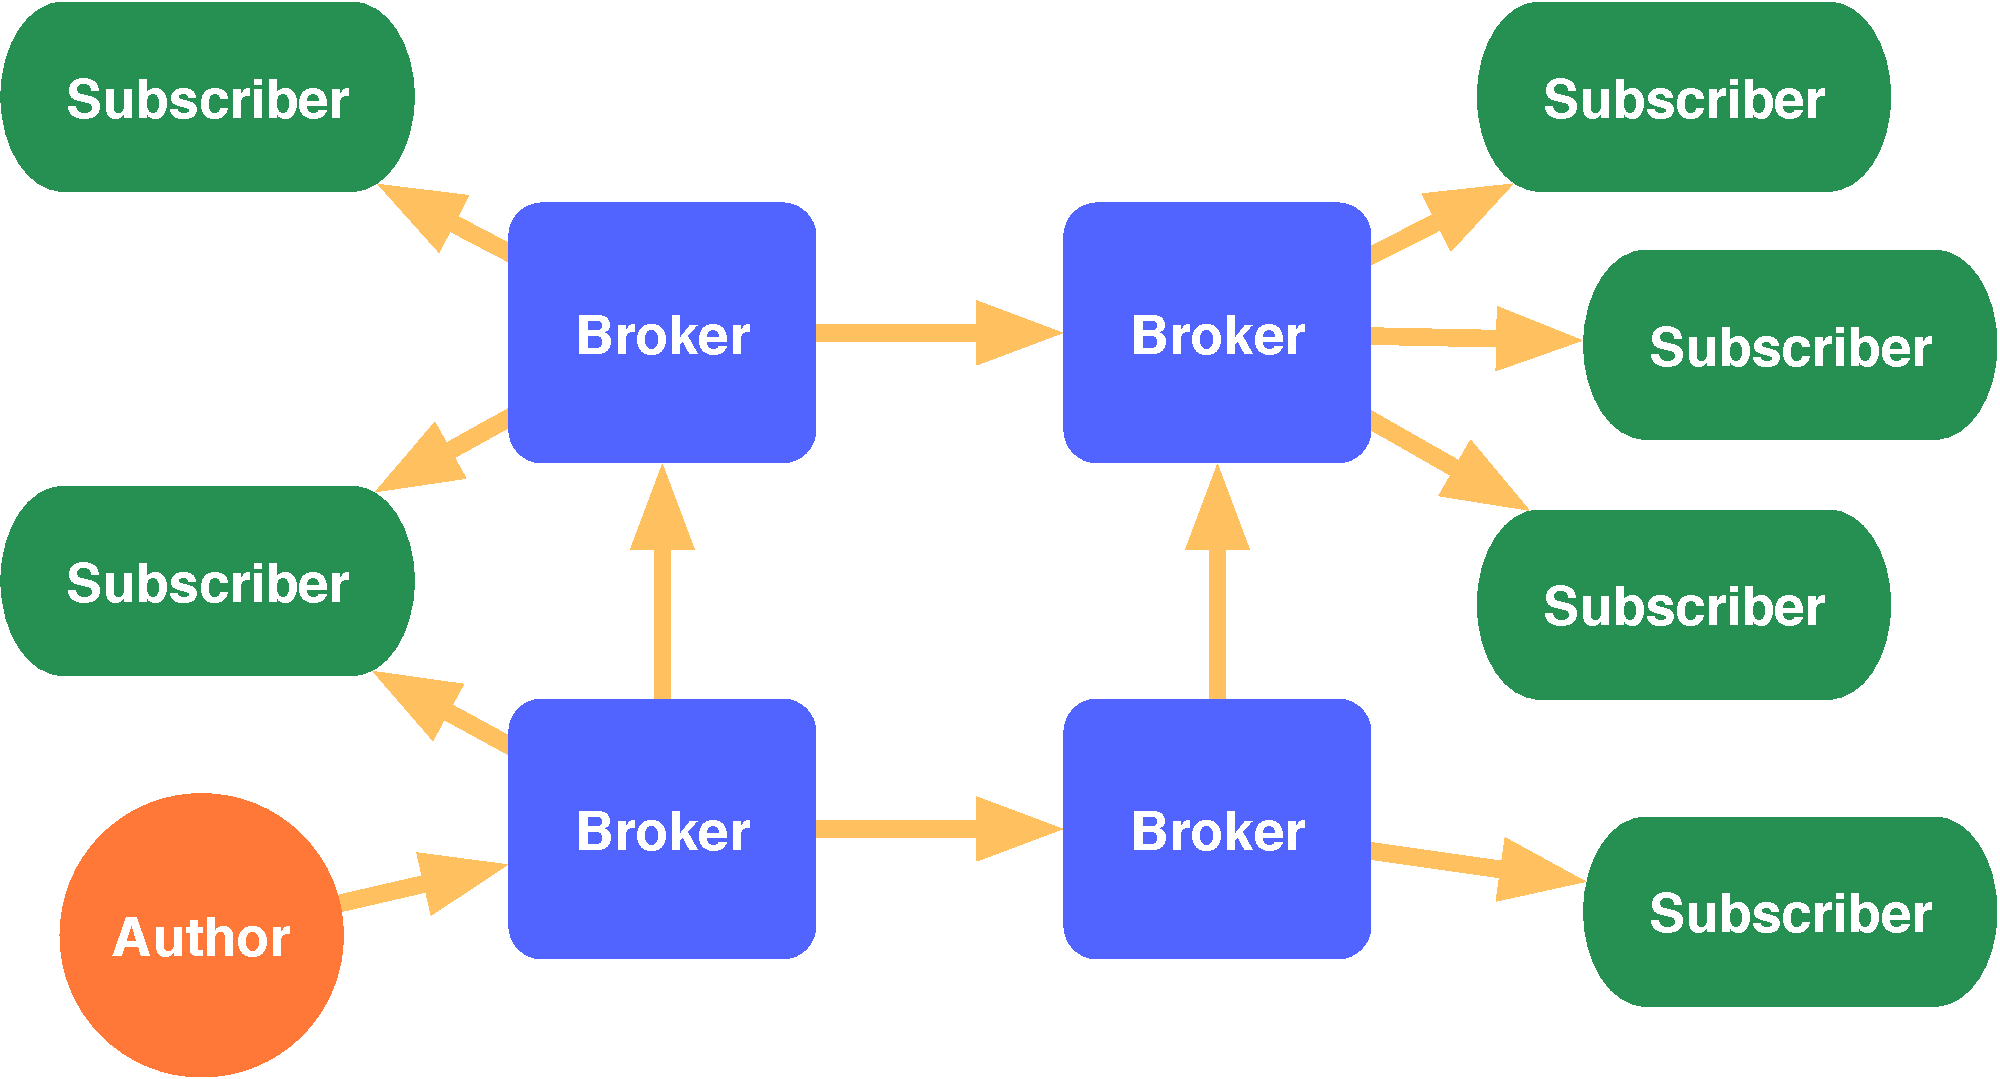
\includegraphics[width=0.7\textwidth]{@FIGURE_OUTPUT_DIR@/vtp.pdf}
  \end{center}

  \caption{An overview of the passage of a VOEvent through a VTP network. The
  arrows indicate data flow. First the event is sent by an author to a single
  broker. This broker then distributes it to all of its subscribers, which may
  include other brokers, which, in turn, redistribute the event until every
  entity on the network has received a copy.  Adapted from
  \citet{Swinbank:2014}.}

  \label{fig:vtp}
\end{figure*}

VTP provides a simple, minimalist system for distributing VOEvents from one or
more authors to a distribute network of potentially interested subscribers. It
builds upon the semantics of VOEvent interchange described in the VOEvent
standard \citep{Seaman:2011}, but includes only those entities which directly
interact by means of the network. To wit, VTP defines the following network
roles:

\begin{description}

  \item[Author]{An author is responsible for creating and publishing one or
  more VOEvents.}

  \item[Subscriber]{A subscriber is interested in receiving the VOEvents
  generated by one or more authors.}

  \item[Broker]{The broker receives VOEvents from other network entities
  re-distributes them to one or more subscribers. In addition, the broker may
  perform ``added value'' on behalf of the subscriber, for example by filtering
  the event stream and forwarding only events of interest, or by annotating
  events with additional information.}

\end{description}

Connections between these entities take place over TCP \citep{Cerf:1974}. The
standard defines three types of connection:

\begin{description}

  \item[Author to Broker]{The author makes a TCP connection to the broker and
  transmits a VOEvent packet. On receipt, the broker sends an acknowledgement.
  The connection is then closed.}

  \item[Broker to Subscriber]{The author opens a TCP connection to the broker,
  which remains open indefinitely. The broker and subscriber send periodic
  ``heartbeat'' messages over the connection to verify that it remains live.
  When the broker receives an event for distribution, it sends it to the
  subscriber over this connection. The subscriber replies with an
  acknowledgement.}

  \item[Broker to Broker]{A broker may subscriber to the output of another
  broker. In doing so, it acts as a subscriber, and the relationship between
  them is as described in ``Broker to Subscriber'', above.}

\end{description}

Note that the the broker-to-subscriber connection remains open at all times,
even when a subscriber has recently received an event. The standard mandates
that the subscriber must always be prepared to receive more events, even while
a previous event is still being processed: otherwise, a backlog of events
waiting to be sent to a particular subscriber could build up and overload the
broker.

By causing brokers to subscriber to the output from other brokers, we can
build extended networks of mutually-interconnected brokers. An author need
only publish to one broker, and ultimately their event id distributed to all
entities on the network. This is not only efficient, it is also robust: the
failure of any given entity can only cause local disruption to the
distribution network. The topology of such a network, and the path a VOEvent
packet might take across it, is shown in Fig. \ref{fig:vtp}.

In addition to passing VOEvent XML documents, VTP defines a ``Transport''
document type. Transport documents are used for the heartbeat messages between
brokers and subscribers and for sending acknowledgement of event receipt. The
documents are kept intentionally short, providing simply a timestamp, an
indication of the originator, and---in the case of a acknowledgement---the
identity of the event being acknowledged.

VTP makes limited provision for securing access to the network: that is, for
limiting the authors and subscribers which may connect to a given broker. The
simplest, albeit least flexible, approach is for the broker to maintain a
``whitelist'' of the IP addresses of entities which are authorized to connect,
and simply drop connections coming from elsewhere. Such a system is convenient
and easy to implement for small networks, but can rapidly become unwieldy as
the list of authorized users grows or as those users need to connect from
multiple addresses. An alternative is therefore suggested in the standard
based on cryptographically signed transport messages, which enable an entity
to securely demonstrate its identity on connection. The means by which these
signatures may be applied is not specified in the VTP standard, which rather
refers to the systems proposed by \citet{Denny:2008}, \citet{Allen:2008} and
\citet{Rixon:2005}. The application of cryptographic signatures to XML
documents is a potentially complex topic, and one to which we return in
\S\ref{sec:security}.

\section{The Design and Implementation of Comet}
\label{sec:design}

Comet\footnote{\url{http://comet.transientskp.org/}} is a freely available,
open source implementation of VTP. It is capable of acting any or all of the
roles within a VTP network: it can receive events from remote brokers (the
subscriber role), receive events from authors and distribute them to
subscribers (the broker role) and it provides a tool which can publish a
VOEvent to a remote broker (the author role). Comet has the twin aims of
acting both as a production-ready event distribution system, which projects
can immediately start using to service their science goals, and as a
convenient system for exploring the characteristics of VTP and exploring and
prototyping future extensions to the protocol. The first aim has already been
met: see, for example, \citet{Staley:2013}. Early results from the second aim
are described in the subsequent sections of this manuscript.

\subsection{Twisted Python and event-driven programming}
\label{sec:design:twisted}

Comet is implemented in Python, and is built atop the Twisted networking
engine\footnote{\url{https://twistedmatrix.com/}}. Twisted enables an
\textit{event-driven} and \textit{asynchronous} style of development which is
extensively used throughout Comet and is fundamental to understanding its
implementation.

Conventionally, we thing of programs as being executed in order: the system
executes the instructions described by the first statement, followed by the
second statement, and so on until the process is complete. Of course,
spreading a process across multiple threads of execution makes the precise
ordering of statements non-deterministic \citep[and, indeed, introduces a whole
new level of complexity in the process;][]{Lee:2006}, but the fundamental
point remains: the aim is to execute the program as rapidly and efficiently as
possible and then exit.

It is obvious that this model does not map well to network based applications.
Consider the ``subscriber'' role in a VOEvent network: it is not rushing to
finish some particular task and then terminate, but rather to continue
listening to the network indefinitely for the arrival of VOEvents, and to
take appropriate action when an event is received. Event-driven programming is
the generalization of this concept: rather than a list of instructions to be
executed sequentially, we define the actions that should be taken in response
to possible events. Twisted then provides an ``event loop'' which waits for
events and calls the appropriate actions when they occur.

\begin{listing}[H]
\begin{minted}[frame=lines]{python}
class VOEventReceiver(Protocol):
  TIMEOUT = 20

  def connectionMade(self):
    setTimeout(self.TIMEOUT)

  def connectionLost(self):
    setTimeout(None)
    close_connection()

  def timeoutConnection(self):
    log.msg("Connection timed out")

  def stringReceived(self, data):
    message = parse(data)
    if is_valid(incoming_message) and \
       message.get("role") in VOEVENT_ROLES:
        log.info("Good message received")
        return_acknowledgement(message)
        process_event(message)
    else:
        log.warning("Bad message received")
    close_connection()
\end{minted}
\caption{An example of an event-driven Twisted protocol, based on Comet's
\texttt{VOEventReceiver}.}
\label{lst:event}
\end{listing}


When talking to the network, Twisted provides the \textit{Protocol} as an
abstraction for managing events. A protocol defines the interaction that a
particular component of the system has with the network. For example, Listing
\ref{lst:event} shows a simplified version of the protocol for Comet's
\texttt{VOEventReceiver}. This is the part of the broker which listens to the
network for submissions from authors. Four separate events are handled by this
protocol:

\begin{itemize}

\item{When a new connection is initiated by an author, the broker sets a
timer on the connection. If no traffic is received, the timer will eventually
reach zero and the connection will be timed-out.}

\item{When a connection is lost, the timeout is aborted.}

\item{When a connection times out, close it.}

\item{When a string is received over the connection, parse it and see if it
can be recognized as a valid VOEvent. If so, return an acknowledgement and
process the newly received event (for example by re-distributing it to
subscribers). If not, log a warning message. Finally, shut down the
connection.}

\end{itemize}

Similar, although often more complex, protocols are defined for all of the
other roles in the system: an author connecting to a broker
(\texttt{VOEventSender}), a broker to a subscriber
(\texttt{VOEventBroadcaster}), and an subscriber to a broker
(\texttt{VOEventSubscriber}).

Event-driven programming provides a convenient abstraction for responding to
network events. However, it does not address issues regarding concurrency. As
described in \S\ref{sec:vtp}, VTP requires that even immediately after
receiving an event subscribers must be ready to accept another: there can be
no delay while the event is ingested. Contrast this with the model described
above and outlined in Listing \ref{lst:event}: here, when an event is
received, each of the functions \texttt{parse()}, \texttt{is\_valid()},
\texttt{return\_acknowledgement()}, \texttt{process\_event()} and
\texttt{close\_connection()} is called in turn.  If these operations are not
assumed to be instantaneous, we must wait for them to complete before
proceeding. While waiting, new events cannot be received.  We are thus in
violation of the VTP standard\footnote{In practice, the implementation of some
of these operations used in the Comet codebase can be assumed to be
effectively instantaneous.  This is safe so long as the time taken to parse is
sufficiently short that no backlog of events waiting to be processed  builds
up and no network timeouts occur.}.

Twisted addresses this problem through the use of \textit{Deferred}s. A
deferred is effectively a promise that processing is underway and that results
will be available in future. We can then queue up other processing tasks (or
``callbacks'') that will be executed when the result of the deferred is
available. For example, we could define a version of
\texttt{parse()}---call it
\texttt{deferred\_parse()}---that, rather than returning an object
representing a parsed version of the VOEvent document, returns a promise to
eventually parse the document in the future and then make it available for
further processing. We can then queue up our other functions to run only when
parsing is complete. For example, see Listing \ref{lst:deferred}, in which we
queue up a number of callbacks to be run when parsing is complete and also add
an ``errback'' which handles logging a message if any of the callbacks fail to
run successfully.

\begin{listing}[H]
\begin{minted}[frame=lines]{python}
def stringReceived(self, data):
  d = deferred_parse(data)
  d.addCallback(is_valid)
  d.addCallback(check_role)
  d.addCallback(return_acknowledgement)
  d.addCallback(process_event)
  d.addErrback(log_failure)
  d.addCallback(close_connection)
\end{minted}
\caption{A version of \texttt{VOEventReceiver.stringReceived()} (shown in
Listing \ref{lst:event}) based on deferred processing.}
\label{lst:deferred}
\end{listing}

Finally, we must implement \texttt{deferred\_parse()}.  Simply returning a
deferred from a function does not prevent it from blocking.  Instead, we
create a dedicated thread which is devoted to parsing the data, and have it
run concurrently with the rest of the application. When that thread completes,
the deferred fires with its result. Conveniently, Twisted makes it easy to
apply this pattern to a blocking function such as our \texttt{parse()}: see
Listing \ref{lst:deferToThread}.

\begin{listing}[H]
\begin{minted}[frame=lines]{python}
from twisted.internet.threads import \
     deferToThread

def deferred_parse(data):
    return deferToThread(parse, data)
\end{minted}
\caption{The implementation of the non-blocking \texttt{deferred\_parse()} function.}
\label{lst:deferToThread}
\end{listing}


Although the examples presented in this section are only intended to be
illustrative, they demonstrate the concepts of asynchronous, event-driven
programming upon which Comet is built and are fundamental to understanding its
operation.

\subsection{Comet architecture}
\label{sec:design:architecture}

Comet is built around the four protocols discussed in
\S\ref{sec:design:twisted}. These enable it to take the part of either side in
each of the three connection types discussion in \S\ref{sec:vtp}. For the
convenience of end users, these are made accessible under two distinct front
ends. In this section, we first introduce those components and describe the
relationship between them, and then discuss how Comet implements some specific
requirements of VTP.

\subsubsection{The components of Comet}
\label{sec:design:components}

The first is \textit{comet-sendvo}. This is a command-line tool which enables
the user to submit a VOEvent to a remote broker. The user is expected to
supply the VOEvent either on standard input or via a reference to the
filesystem; \textit{comet-sendvo} transmits it to the specified destination
using the \texttt{VOEventSender} protocol and shuts down.

Processing a single event and then exiting is an appropriate model for an
author, but is not the behaviour required of a broker or subscriber. Rather,
these tools must remain active, continuing to receive and process VOEvents
until the user shuts them down. To support this mode of operation, Comet can
run as a ``daemon'', or background process. The Comet daemon can:

\begin{enumerate}

  \item{Accept submissions from authors (including, of course, \textit{comet-sendvo});}

  \item{Subscribe to event streams from one or more remote brokers;}

  \item{Distribute events received (whether by direct author submission or by subscription) to its own subscribers;}

  \item{Perform arbitrary actions upon the events received.}

\end{enumerate}

A single Comet daemon is capable of performing any or all of these actions,
depending upon configuration: it is not necessary to start separate ``broker''
and ``subscriber'' daemons, for example.

Both \textit{comet-sendvo} and the Comet daemon make extensive use of the
facilities provided by Twisted for event-driven and asynchronous programming,
as well as its support for logging and daemonization. They are exclusively
command-line driven, and do not rely on configuration files.

\subsubsection{Event de-duplication}
\label{sec:design:dedup}

As described in \S\ref{sec:vtp} it is possible to build a mutually
interconnected ``mesh'' of brokers to efficiently and reliably distribute
events to a large number of subscribers. However, this runs the risk that
events could continue ``looping'' on the network indefinitely, as two or more
brokers which subscribe to each other's feeds repeatedly exchange the same
event. To avoid this problem, Comet refuses to process any given event more
than once: if a newly received event is the same as one which has been
previously seen, it is simply dropped without being further distributed.

In order for this approach to be effective, it is necessary to define what it
means for an event to be ``the same''. In particular, due to the nature of
XML, it is possible for exactly the same information about an event (the
``infoset'') to be encoded in multiple different, but all equally valid, XML
documents. At the simplest level, this is because XML is (for the most part)
white space agnostic---new lines or spaces can be inserted without changing
the meaning of the document. The question becomes more complex, though, when
we consider the various versions of the VOEvent standard. Version 2.0
\citep{Seaman:2011} is current, but the previous version
\citep[1.1;][]{Seaman:2006} is still in use by some systems. If the same
information about the same astronomical event is encoded in a VOEvent 2.0
document and a VOEvent 1.11 document, are these ``the same''?

This question is particularly pertinent because this situation is exactly that
which exists in practice: since
2012\footnote{\url{http://gcn.gsfc.nasa.gov/admin/voevent_version20_available.txt}},
NASA GCN has issued both version 1.1 and version 2.0 VOEvents containing the
same information.

\citet{Seaman:2011} requires that each VOEvent carry an
IVORN\footnote{International Virtual Observatory Resource Name} which ``will
stand in for a particular packet''. It is this IVORN that is used to identify
events in the context of references and citations, for example. There has been
some
debate\footnote{\url{http://www.ivoa.net/pipermail/voevent/2012-March/002836.html}}
as to whether IVORNs uniquely identify a particular infoset or a particular
representation thereof: this is not currently well defined by the relevant
documentation. In the case of the events issued by GCN, a single IVORN is used
to describe both the version 1.1 and the version 2.0 VOEvent packets: this
provide a \textit{de facto} standard that the IVORN identifies the infoset.

VTP makes no distinction between the versions of VOEvents which it transmits:
the same protocol may be used for version 1.1, or 2.0, or putative future
versions. However, the consumer of a particular VOEvent may well have a
toolchain that is tuned to work with one particular standard. In other words,
authors may wish to use a VOEvent network to distribute multiple different
versions of the same event, while subscribers may depend on receiving a
specific representation of that event. In short, if an author submits version
1.1 and version 2.0 representations of an event, it would not be appropriate
for a broker to regard them as duplicates and discard one of them. The only
possible conclusion is that the IVORN is not a suitable means of identifying
unique events for the purposes of de-duplication.

Comet therefore regards events as duplicates only if they are bit-for-bit
identical with an event which has been seen before. This is determined by
calculating the SHA-1 \citep{Eastlake:2001} cryptographic hash of every event
which is seen by a Comet daemon and storing it, together with the time and
date at which the event was seen, in a DBM-style persistent
database\footnote{``DBM-style'' databases provide mappings between ``keys''
and ``values'' in the manner of an associative array. Various libraries
implementing this style of database exist exist; Comet uses Python's
\texttt{anydbm} interface, which automatically chooses a particular
implementation based upon the platform on which it is running.}. When an event
is received, its SHA-1 hash is calculated and compared against the contents of
the database to establish if it has been seen before.

Each individual SHA-1 hash is stored as 40 bytes, plus a further 13 bytes are
used to records the timestamp. The total storage requirement is therefore very
modest. However, on a busy broker processing many events, the database could
grow to a significant size, wasting resources and slowing down access.
Therefore, Comet periodically removes all events older than 30 days from its
database. Duplicates issued more than 30 days after the original event will
therefore not be detected; however, an event loop with a period of 30 days or
longer poses no threat to the integrity of the network.

It should be noted that this de-duplication scheme requires that all entities
on the network forward events unchanged: even an apparently inconsequential
change to an event packet which results in a valid event encoding the same
infoset as before would result in a different SHA-1 hash for the event. The
current VTP standard implies but does not absolutely require this behaviour:
see \S\ref{sec:futurevtp} for further discussion.

\subsubsection{Security and whitelisting}
\label{sec:design:security}

The released version of Comet at the time of writing (1.1.0; see
\ref{sec:avail}) does not implement an authentication scheme based on
cryptographic signatures as described in \S\ref{sec:vtp}. Work is ongoing on
prototyping such a scheme using Comet as a test-bed: this is described in
\S\ref{sec:security}.

When acting as a broker, Comet includes the ability to check authors
submitting events against a whitelist of IP addresses. Multiple disjoint
ranges of addresses to whitelist may be specified using CIDR notation
\citep{Fuller:1993}, making the system very flexible.

Comet does not currently provide built-in whitelisting support for
subscribers. However, equivalent functionality is available though the use of
an operating system level packet filter.

\subsubsection{Acting on events received}
\label{sec:design:plugin}

Just receiving a VOEvent and optionally re-distributing it is of limited
practical value: ultimately, some recipient of the event will wish to take
action based upon it. The algorithms which may be employed to determine
whether a particular event is worth of follow-up are dependent on the
particular science goals of the recipient, are potentially complex, and are
certainly outside the scope of this manuscript. Since it is not possible to
anticipate the requirements of the end user in a universally applicable way,
Comet rather seeks to be easily adapted to each particular use case. Two
mechanisms are provided to make this possible.

The simplest option is that when a new event is received, Comet can spawn an
external process and provide the text of the event to it on standard input.
The process is run asynchronously, so that potentially lengthy processing jobs
can be run on events without interrupting Comet's operation. Comet monitors
the execution of the process and logs a warning if it is unsuccessful (that
is, if it exits with a status other than \texttt{0}), but otherwise has no
control over the processing performed.

In some circumstances, the user may wish for more control than is provided for
by passing events to another process. Comet therefore makes it possible to
write \textit{plugins}, which can be loaded into the daemon at run time.
Users write plugins in Python, implementing a standard interface. Plugins
provide a \texttt{\_\_call\_\_()} method which is invoked with the contents of
an event whenever one is received. An example is shown in Listing
\ref{lst:plugin}.

\begin{listing}[H]
\begin{minted}[frame=lines]{python}
from zope.interface import implementer
from twisted.plugin import IPlugin
from comet.icomet import IHandler

# A plugin implements the IPlugin
# and IHandler interfaces
@implementer(IPlugin, IHandler)
class ExamplePlugin(object):
    # The "name" attribute is used to refer
    # to the plugin on the command line.
    name = "example"

    # The "__call__()" method is invoked
    # when a new event is received.
    def __call__(self, event):
        print "Event received"

# The plugin must be instantiated before use.
example_plugin = ExamplePlugin()
\end{minted}
\caption{A simple example of a Comet event handling plugin. This plugin prints
a message whenever a new event is received.}
\label{lst:plugin}
\end{listing}

Comet automatically probes for all available plugins and makes them available
as command line arguments, so the user can specify which plugins are required
when the daemon is started. If required, plugins may also define
user-configurable options by implementing the \texttt{IHasOptions} interface;
these are also exposed on the command line.

\section{Filtering events}
\label{sec:filter}

Next generation telescopes such as LSST promise to detect and announce
transients using VOEvent at a rate of millions of events per night
\citep{Kantor:2014}. It is unlikely that most individual subscribers will have
a use for all of these events. Winnowing that event stream down so that each
subscriber receives only those events which are of direct relevance to them is
both efficient in terms of resource usage, as fewer events need to be
transported to and processed by the subscriber, but also enables subscribers
to focus simple, well-targeted systems that address their science goals,
rather than attempting to devise efficient ways to process millions of VOEvent
packets.

Efforts to develop intelligent systems for alerting users only of those events
which are of relevance to them are ongoing, and will continue into the future
\citep{Williams:2009, Matheson:2014}. Comet contributes to this effort by
introducing a powerful XPath \citep{Clark:1999} based filtering system.

\subsection{XPath queries}

XPath is a language for selecting parts of and computing values over an XML
document. XPath expressions may return one of four different result types:

\begin{itemize}
  \item{A Boolean value;}
  \item{A floating point number;}
  \item{A textual string;}
  \item{A set of XML ``nodes'', representing parts of the document.}
\end{itemize}

XPath expressions enable users to specify complex queries, including testing
the values of arbitrary elements or attributes specified in the document and
combining those tests with Boolean logic. A complete reference is outside the
scope of this manuscript, but some examples may serve to illustrate the
possibilities.

Starting with string matching, \mint{xml}|//Who/Author[shortName="VO-GCN"]|
returns a set of all nodes in the document which list the author's ``short
name'' as \texttt{VO-GCN}. More complex matches can use functions, such as
\mint{xml}|//How[contains(Description, "Swift")]| which returns the set of all
nodes which mention ``Swift'' in the context of a describing how the data was
obtained. Numerical comparisons are also possible:
\mint{xml}|//Param[@name="Sun_Distance" and @value>40]| provides the set of
all parameters called \texttt{Sun\_Distance} with a numerical value greater
than 40.

These expression can be combined, so that for example
\begin{minted}{xml}
//How[contains(Description, "Swift")] or
  ( //Param[@name="Sun_Distance" and @value>40]
    and //Who/Author[shortName="VO-GCN"]) )
\end{minted}
returns a Boolean value which is true if the event either mentions ``Swift''
or both has a \texttt{Sun\_Distance} parameter greater than 40 and originates
from GCN, and false otherwise.

\subsection{Integration with Comet}

Comet makes it possible for a subscriber to supply one or more XPath
expressions to a broker. When the broker receives an event, it evaluates each
expression over the event, and only forward it to the subscriber if at least
one of the expressions evaluates produces a positive result.

Comet takes the result returned by XPath and applies Python's \texttt{bool()}
built-in function to determine if the result is ``positive''. For example, the
values \texttt{True}, \texttt{1} and \texttt{"string"} (the Boolean true
value, a non-zero number and a non-empty string) as well as a non-empty node
set are all positive, while \texttt{False}, \texttt{0} and \texttt{""}
(Boolean false, the number 0 and an empty string) and the empty node set are
``negative'' results.

VTP provides no standardized method for a subscriber to communicate their
filter preferences to the broker. Comet works around this by overloading the
Transport message system provided by VTP and described in \S\ref{sec:vtp}.
According to the VTP specification, it is legal for a subscriber to send a
Transport message of class \texttt{authenticationresponse} and with arbitrary
metadata embedded at any time during a VTP session. Comet looks for XPath
expressions encoded in this metadata and installs them as filters for the
subscriber; other brokers which comply with the protocol but do not support
this form of filtering should simply ignore the message.

\section{Performance}
\label{sec:perf}

Comet not been designed primarily for performance: at time of writing, typical
VOEvent brokers are processing perhaps a few hundred events per day, so the
total computational and storage demands are extremely modest. However, it is
informative to consider both how Comet and the VTP architecture scale to cope
with the millions of events per night promised by future facilities such as
LSST. In this section, we quantify both the number of events Comet is capable
of processing, the latency which it introduces to the event stream, and the
number of subscribers which a broker can conveniently service.

\subsection{Test system configuration}
\label{sec:perf:system}

The basic configuration of all tests below consists of one or more authors
connecting to a broker and sending it events which the broker then distributes
to one or more subscribers. The processes acting as authors, brokers and
subscribers were all run on the same modest desktop system, based on an Intel
Core i7 940 CPU\footnote{Four cores with two threads each running at
2.93\,GHz.}
and 8\,GiB RAM. Storage was provided by two 7200\,RPM magnetic disks
configured as a RAID-0 array. The system was running Debian GNU/Linux with kernel
version 3.13.

In realistic scenarios, VOEvent authors, brokers and subscribers would not
co-exist on the same system. However, providing many separate test systems was
impractical, and exchanging events over the public internet (or even over a
local network) introduces an extra layer of uncertainty in terms of packet
latency. Instead, the various processes being tested were run in isolated
process containers using Docker\footnote{https://www.docker.io/}. Docker-based
containers operate in much the same way as traditional virtual machines,
except they incur no virtualization overhead, directly addressing the same
kernel as the host system, but only able to communicate with each other over
(virtual) network interfaces.  Within each container a minimal
Ubuntu\footnote{\url{http://www.ubuntu.com/}} Linux 12.04 system was
installed, providing Python 2.7.3 and Twisted 11.1.0. The ``Dockerfile'' used
to create exactly the configuration used for testing is available from the
Comet repository; see \S\ref{sec:avail}.

\subsection{Latency}
\label{sec:perf:latency}

For certain science cases, maximizing the scientific relevance of follow-up
observations requires extremely rapid response. For example, identifying
precursors of fast radio bursts \citep{Thornton:2013} would require action on
a timescale a tens of milliseconds. It is therefore important that the VOEvent
transport system does not introduce excessive latency to the dissemination of
event notifications.

For the purposes of this discussion, we define the ``latency'' of a VOEvent as
the time elapsed between its creation by an author and the instant at which it
has been received by a subscriber and that subscriber is in a position to take
action (using the strategies described in \S\ref{sec:design:plugin}) based
upon it.

In this test, we measure the latency introduced by passing a VOEvent from an
author through a Comet broker and on to a Comet-based subscriber.

\subsubsection{Test setup}
\label{sec:perf:latency:setup}

\begin{listing*}
\begin{minted}[frame=lines]{xml}
<?xml version='1.0' encoding='UTF-8'?>
<voe:VOEvent
  xmlns:voe="http://www.ivoa.net/xml/VOEvent/v2.0"
  xmlns:xsi="http://www.w3.org/2001/XMLSchema-instance"
  ivorn="ivo://comet.broker/test#TestEvent-2014-03-31T16:16:37" role="test" version="2.0"
  xsi:schemaLocation="http://www.ivoa.net/xml/VOEvent/v2.0
    http://www.ivoa.net/xml/VOEvent/VOEvent-v2.0.xsd"
  >
<Who>
  <AuthorIVORN>ivo://comet.broker/test</AuthorIVORN>
  <Date>2014-03-31T16:16:37.040340</Date>
</Who>
  <What>
    <Description>Broker test event generated by Comet 1.1.0.</Description>
    <Reference uri="http://comet.transientskp.org/"/>
  </What>
<voe:VOEvent>
\end{minted}
\caption{An example of the form of VOEvent used for benchmark testing. The
\texttt{ivorn} attribute of the \texttt{VOEvent} element and the \texttt{Date}
element were automatically generated and reflect the time at which the packet
was created.}
\label{lst:testmessage}
\end{listing*}

A script was used to generate 3000 individual VOEvent packets and submit them
to a broker at intervals of 0.3 seconds.  Each packet was compliant with the
VOEvent schema, but carried a relatively small payload amounting to little
more than a timestamp reflecting when the event was created: see Listing
\ref{lst:testmessage} for an example.

A plugin (\S\ref{sec:design:plugin}) was written which, whenever an event of
the form described above is received, compares the timestamp in the event with
the current time, and saves the difference to a log file. This plugin was
enabled on a subscriber, which was connected to the broker.

Both the benchmarking script and the plugin described are available from the
Comet repository (\S\ref{sec:avail}).

\subsubsection{Results}
\label{sec:perf:latency:results}

\begin{figure}
  \begin{center}
  \includegraphics[width=\columnwidth]{@FIGURE_OUTPUT_DIR@/latency.pdf}
  \end{center}

  \caption{Fraction of events received at a given latency (time between
  generation by the author and processing by the subscriber, as described in
  \S\ref{sec:perf:latency}. The uppermost plot reflects the default
  configuration; the central plot uses Twisted's \texttt{epoll()} based
  reactor; the bottom plot uses \texttt{epoll()} and stores the event database
  in memory.}

  \label{fig:latency}
\end{figure}

The distribution of latencies among the received events when this test was run
in the default configuration is shown in the top panel of Fig.
\ref{fig:latency}. The mean latency was 0.022\,s with a standard deviation of
0.011\,s; the longest recorded latency for any event was 0.171\,s.

As described in \S\ref{sec:design:twisted}, Twisted provides an event-driven
framework. The core of this framework is the ``reactor'', which provides a
uniform interface to event handling across the platforms upon which Twisted
can run. The internal implementation of the reactor itself can vary from
platform to platform to most efficiently take advantage of the facilities
available to it.

The default reactor implementation used by Twisted on the system used for
testing is based on the \texttt{poll()} system call \citep{Posix1:2013}.
However, modern Linux systems provide the alternative \texttt{epoll()} call
\citep{Kerrisk:2014} which provides a more efficient alternative. Twisted
provides a reactor which is based upon \texttt{epoll()}. In the middle panel of
Fig. \ref{fig:latency} the same experiment was repeated, but with both broker
and subscriber based on this alternative reactor. This provided a somewhat
improved mean latency of 0.019\,s with a standard deviation of 0.011\,s, and a
reduced maximum latency of 0.130\,s.

As described in \S\ref{sec:design:dedup}, Comet stores a database of the
arrival times and SHA-1 hashes of each event it processes, both at the broker
and at the subscriber. This data is regularly written the filesystem as Comet
is running, and must be searched for duplicates every time a new event is
received. Accessing disk storage involves a significant overhead, so a new
memory-based filesystem was created based on \texttt{tmpfs}
\citep{Kerrisk:2014} and both broker and subscriber were configured to store
their event databases here. This storage is entirely RAM-based, so avoids the
extra delays in writing to disk. Of course, the RAM technologies typically
used in modern systems are inherently volatile, and the event database would
not survive if the system were powered down and rebooted: whether this risk is
appropriate in a production deployment would be a matter of judgement.

The results based on the \texttt{tmpfs} filesystem are shown in the bottom
panel of Fig. \ref{fig:latency}. Clearly, these latencies are both lower (mean
0.0063\,s, maximum 0.013\,s) and more consistent (standard deviation
0.00033\,s) than the previous tests.

An overhead of no more than around ten milliseconds is comparable to that
which might be expected from network delays over short links, and is unlikely
to be of significance in most astronomical applications. For the rest of the
tests presented in this manuscript, we continue to adopt the \texttt{epoll()}
and \texttt{tmpfs} configuration described here.

\subsection{Number of subscribers}

In order to meaningfully act as a distribution, rather than simply a
forwarding, system, and certainly in order to enable the construction of
extended networks of interconnected brokers, it is necessary that a single
Comet broker be able to serve many subscribers simultaneously. Here, we
measure how latency increases as more subscribers are connected to the the
broker.

\subsubsection{Test setup}

Using the same script as described in \S\ref{sec:perf:latency:setup}, 1000
test events were submitted to a broker. The number of clients connected to
that broker was increased at logarithmic intervals (1, 2, 4, ...). Each client
recorded the latency of each event received to a log file.

Each Comet process takes approximately 32\,MB of memory, used to hold the
Comet code itself, the associated libraries, the Python interpreter, and the
overhead associated with the Docker container. The test system contained 8\,GB
RAM. When testing with 256 subscribers, the machine ran out of memory and
started to swap to disk. This set an upper bound on the number of subscribers
which could be tested.

\subsubsection{Results}

\begin{figure}
  \begin{center}
  \includegraphics[width=\columnwidth]{@FIGURE_OUTPUT_DIR@/subscribers.pdf}
  \end{center}

  \caption{Event latency as a function of subscriber count. The solid line
  shows the mean latency across all events and all subscribers; error bars
  indicate the standard deviation. The dashed lines indicate the maximum and
  minimum event latency recorded.}

  \label{fig:subscribers}
\end{figure}

Figure \ref{fig:subscribers} shows the event latency as a function of
subscriber count. The latency increases gradually with increasing subscriber
count, from a mean of 0.0063\,s for a single subscriber to 0.0931\,s for 256
subscribers, the highest number tested: even at this level, the mean latency
was less than 0.1\,s. The maximum latency rose to a peak of 0.49\,s.

A latency of around 0.1\,s is comparable to a long range (e.g. transatlantic)
network round trip times and is at a level where it may start to impact on the
most time-critical astronomical applications (\S\ref{sec:perf:latency}).

Other than a slowly increasing latency, the Comet system showed no
ill effects of handling a large number of subscribers: neither memory nor CPU
usage of the broker showed excessive growth. If the latency were acceptable
for the science application, there would be no difficulty in serving 256
subscribers in a production mode.

For servicing extremely large numbers of clients while minimizing latency a
tree-like structure could be established. For example, serving 8 subscribers
introduced a mean latency of 0.0093\,s. If each of those 8 subscribers
redistributed the event to a further 8 clients, we might expect a total
latency on the order of 0.02\,s to reach 256 clients; if the tree were
extended to ten levels we might expect to reach $8^{10}$ ($\sim 10^9$)
subscribers with 0.1\,s latency.

\subsection{Total throughput}
\label{sec:perf:total}

Next-generation facilities will announce transients at rates far outstripping
those seen at present. Notably, LSST is predicted to peak at rates of
$3\times10^7$ events per night \citep{Kantor:2014}: assuming those events are
evenly spaced over a 12 hour period, this is equivalent to nearly 700 events
per second.

Here, we measure how the event rate processed by the Comet broker running on
the test system.

\subsubsection{Test setup}
\label{sec:perf:total:setup}

A script was used to generate 10000 individual VOEvent messages, which were
stored in RAM. After all events had been generated, the author started
submitting them to a Comet broker which had a single subscriber attached. The
total time taken by the author from the start of the submission of the first
event to the closing of the connection after the submission of the last event
was measured by recording its running time. The total time from the receipt of
the first event to the receipt of the last event by the subscriber was
measured by taking the difference between the latest and the earliest
timestamps recorded in the event database (\S\ref{sec:design:dedup}). These
times are then converted into an per-second event rate.

The number of concurrent connections between the author and the broker was
varied logarithmically. For each number of connections, the experiment was
repeated 10 times.

\subsubsection{Results}
\label{sec:perf:total:results}

\begin{figure}
  \begin{center}
  \includegraphics[width=\columnwidth]{@FIGURE_OUTPUT_DIR@/throughput.pdf}
  \end{center}

  \caption{At top, the mean throughput of events as transmitted by
  the author and as received by the subscriber as a function of number of
  concurrent connections from author to broker. The central panel shows the
  standard deviation of the measured rates. The number of events which were
  not successfully received by the subscriber is shown at the bottom.}

  \label{fig:throughput}
\end{figure}

Figure \ref{fig:throughput} shows the how the event rate measured at both
author and subscriber varies with the number of concurrent connections. With a
single connection a rate of 283.7 events/second at the author and 283.8
events/second at the subscriber is achieved. This increases to a peak of 519.2
events/second at the author and 534.2 events/second at the subscriber with 64
concurrent connections; after this, increasing he number of connections causes
the overall throughput to drop. The standard deviation of the measured rate is
also plotted: the throughput is relatively stable at low connection counts,
but substantial variations are seen with 256 and 512 concurrent connections.

At the highest connection counts, the rate is not only seen to drop
substantially, but also some events are lost in transit: at the end of the
test, the subscriber had received fewer than 10000 VOEvent packets. Since the
throughput was lower at these rates, and since reliable transmission is
essential, concurrency levels higher than 512 connections were not
investigated.

These results may be explained by considering the balance between the
per-connection overhead and the compute load on the broker. Since each event
is delivered by making a new connection to the broker (as per the protocol
described in \S\ref{sec:vtp}) there is a per-event overhead due to creating
and tearing down the connection (\S\ref{sec:perf:highlatency} discusses some
of the overheads in managing TCP connections). At low connection counts, this
latency dominates; as the concurrency increases, the throughput is dominated
by the broker load.

At the highest connection counts, the configuration of the Linux kernel's
networking stack comes in to play. Large numbers of short lived connections
are a relatively uncommon phenomenon, and the standard configuration of the
Linux kernel is not optimized to handle them efficiently. Indeed, at very high
connection counts, the kernel logged warnings that it was was under a
``\textsc{syn} flood'' attack \citep{CERT:1996}. Under this load, connections
may be dropped or rejected by the kernel, leading to events never reaching
their destination, as seen in the lowest panel of Fig. \ref{fig:throughput}.
Many options within the kernel may be tuned to improve its performance under
these network loads. However, since the peak throughput was already limited by
Comet's CPU requirements at lower connection counts, they were not
investigated here.

It is worth noting that, at low connection counts, the throughput from author
to broker and from broker to subscriber were effectively identical, but they
began to diverge as the concurrency increased. This is again due to the
per-connection overhead: since the connection from the broker to the
subscriber is permanently kept open, it is significantly more efficient, and
provides a continuously-available high bandwidth connection. At high
connection counts the latency involved in servicing many connections means
that such high bandwidths cannot be achieved here.

Without special tuning, the peak throughput of over 500 event/second is over
70\% of that required to service the peak event rate predicted from LSST.
Note, though, this test was limited by CPU performance on desktop-class
hardware that will be substantially more than a decade old before LSST is
commissioned. Further, the predictions refer to a peak rate, not sustained
production. In these terms, then, servicing an LSST event stream with a VTP
based broker seems plausible---although it is worth emphasizing that the
events used in this benchmark did not carry a scientific payload, and hence
are likely significantly smaller than those which might be produced by LSST.

\subsection{High-latency connections}
\label{sec:perf:highlatency}

\begin{figure}
  \begin{center}
  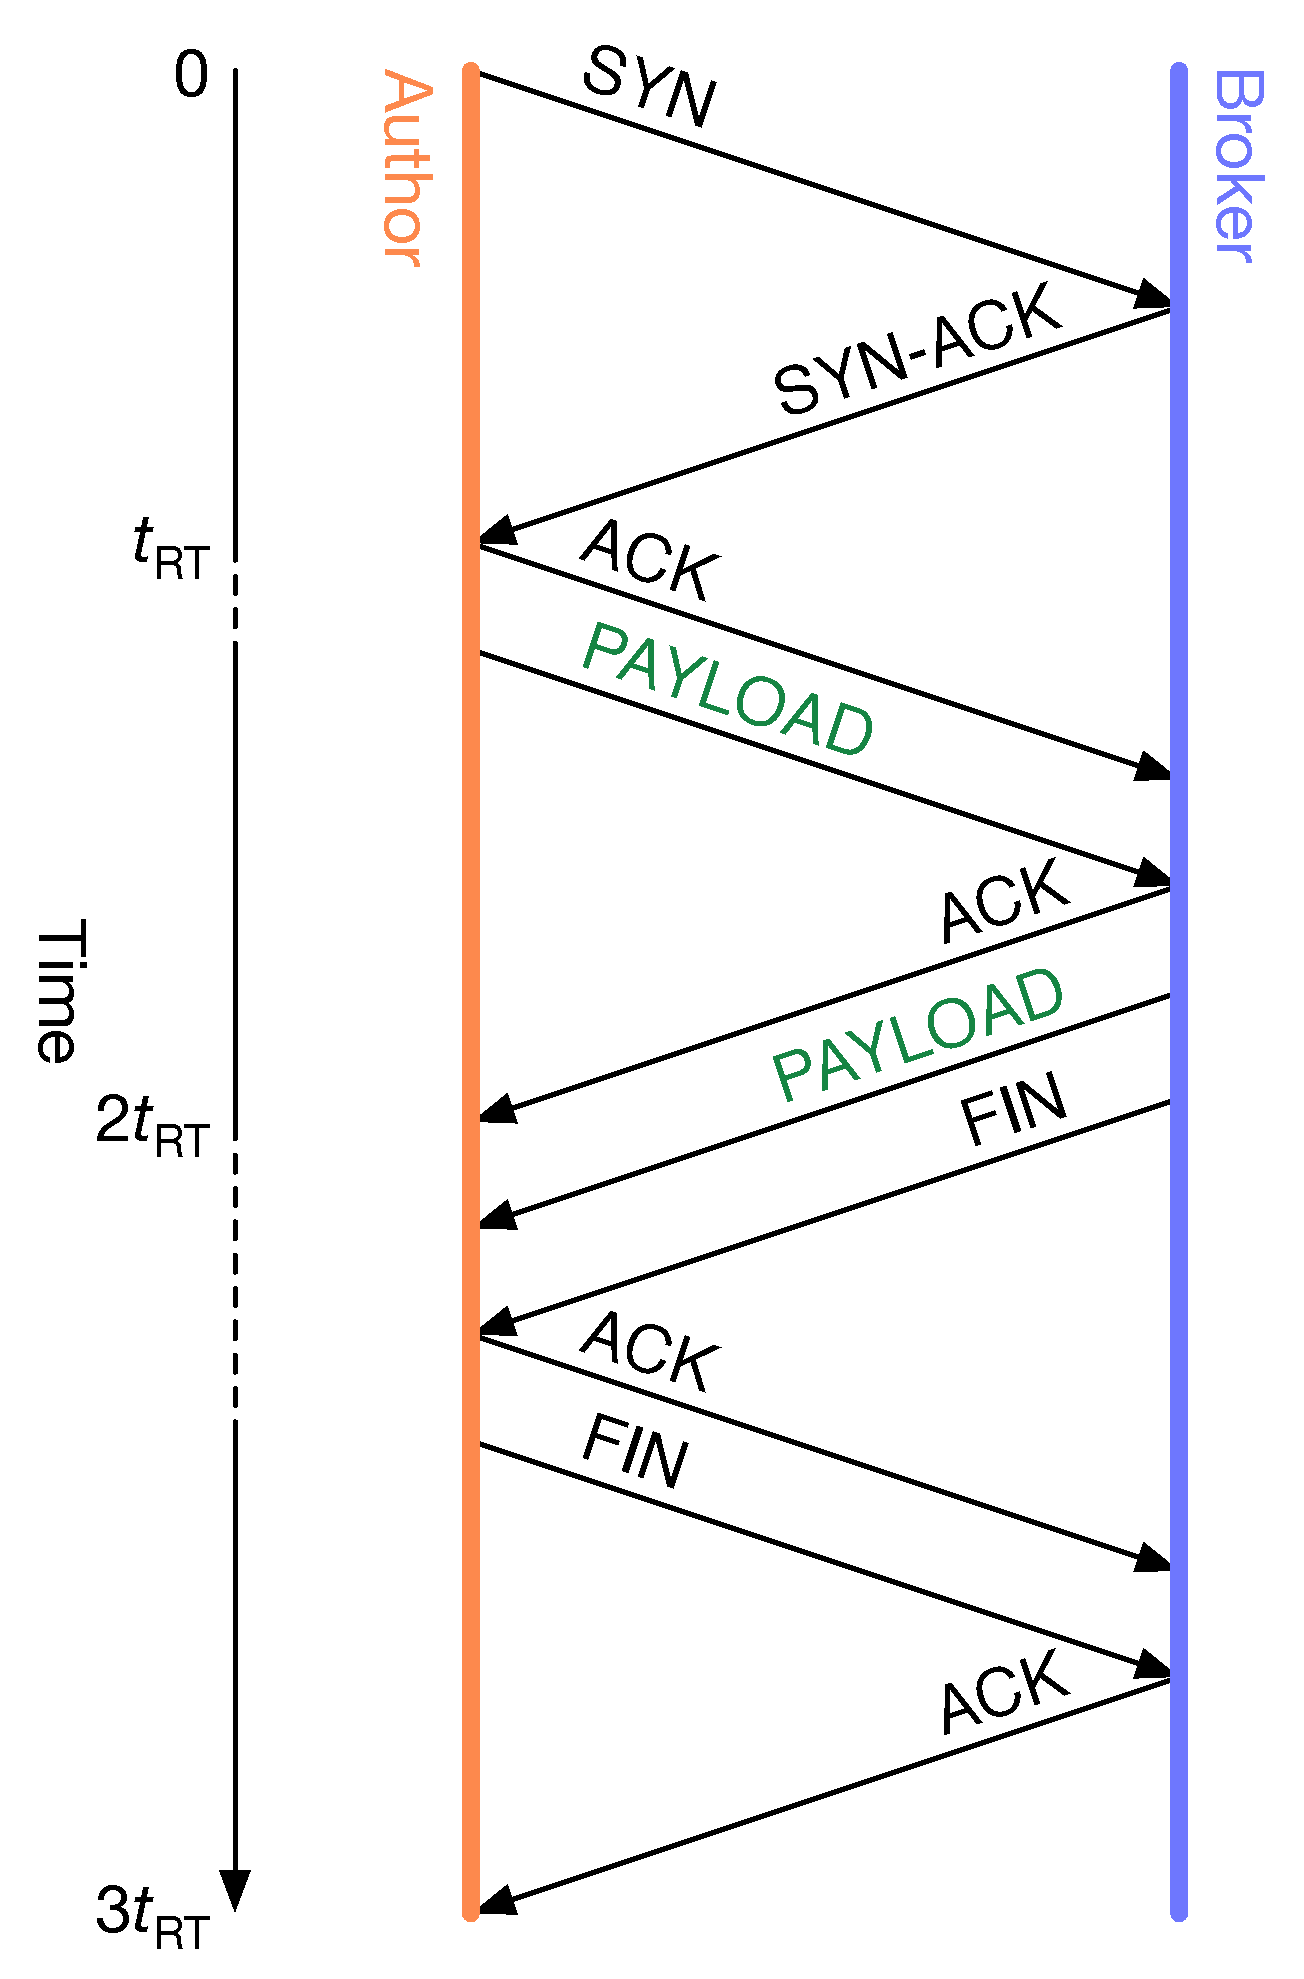
\includegraphics[width=0.7\columnwidth]{@FIGURE_OUTPUT_DIR@/tcp.pdf}
  \end{center}

  \caption{The complete packet exchange as an author uploads a VOEvent to a
  broker. Packets with specific flags set have those flags indicated in black.
  Packets containing payload data (a VOEvent or a Transport message) are
  labelled in green.  Time increases down the diagram. The network round trip
  time is denoted by $t_\mathrm{RT}$. A dashed time axis indicates packets
  being sent with no interval between them. For example, at time
  $t_\mathrm{RT}$ the author sends \textsc{ack} immediately followed by
  VOEvent data.}

  \label{fig:tcp}
\end{figure}

Astronomical observatories are frequently located in remote locations: in
deserts, on mountain tops, and so on. The geographic isolation of these
facilities often results in their having poor internet connections. Even if
high-bandwidth networking is arranged specifically to service the observatory,
network latencies are likely to be high.

It is reasonable to suppose that preliminary data analysis for such an
observatory would be performed on-site, rather than attempting to ship large
volumes of raw data out of a remote location. Further, it would not be
practical for large numbers of external clients to connect inwards to a
VTP broker running at the observatory. Therefore, we we assume that the events
are generated by a VOEvent author on site, then shipped using VTP to a remote
broker for public distribution.

Assuming 10 million are issued by the observatory per night and each event
has a size of around 10\,kiB, a total of 100\,GiB of event data might be
created. Given that long range multi-gigabit per second connections are widely
available, the total amount of data to be transmitted is unlikely to be
intractable.

Network latency, however, presents a further problem. As described in
\S\ref{sec:vtp}, each event must be submitted by the author initiating a new
connection to the broker, submitting the event, waiting for an
acknowledgement, and then closing the connection. Sending the event and
waiting for acknowledgement involves a network round-trip.  However, data is
transmitted over TCP \citep{Cerf:1974}, we use the standard TCP mechanisms for
creating and terminating connections, each of which involves another network
round trip. This process is illustrated in Fig. \ref{fig:tcp}: the complete
transaction involved in submitting a single event to the broker, given a
network round trip time of $t_\mathrm{RT}$, takes $3 t_\mathrm{RT}$. In
practice, after transmitting the final \textsc{fin} packet, the author may
assume that the connection is closed without waiting for a response, and hence
initiate a new connection, so the figure of $2 t_\mathrm{RT}$ describes the
interval between connection attempts.  Assuming that events are sent in
sequentially, and given a round trip time of, say, 200\,ms, this would limit
the total number of events which may be sent in a 12 hour period to 86400, far
short of the rates discussion in \S\ref{sec:perf:total}. However, the same
section also demonstrated that events may be sent concurrently over multiple
connections. Here, we investigate to what extent that approach can mitigate
this issue.

\subsubsection{Test setup}

Events were generated, sent the the broker, and thence onwards to a single
subscriber as per \S\ref{sec:perf:total:setup}, and times were measured in
exactly the same way. Connection counts were again increased logarithmically.
Given the relative stability of the throughput (at least for modest connection
counts) shown in Fig \ref{fig:throughput}, a single set of 10000 events was
sent for each level of concurrency.

Link-level network latency was simulated using NetEm \citep{Hemminger:2005},
the network emulation functionality available as part of the Linux kernel.
Given a (virtual, in this case) network device named \texttt{vethXXX}, a
delay of \texttt{YYY}\,ms may be added to each packet sent through it by
running:
\begin{minted}{sh}
tc qdisc add dev vethXXX root netem delay YYYms
\end{minted}
Note that this delay applies only to packets sent through the interface: no
delay is applied to packets received at the interface. To simulate a symmetric
network delay using this approach, it would therefore be necessary to add a
latency of $t_\mathrm{RT} / 2$ at both the author and the subscriber
interfaces. However, this is complicated by the fact that the subscriber also
communicates with the broker over its interface. Therefore, instead the whole
delay was applied to the output of the author. Given the symmetric nature of
Fig. \ref{fig:tcp}, the observed effect is identical.

\subsubsection{Results}

\section{Authentication}
\label{sec:security}

For many applications involving VOEvents, it is important to be certain of the
authenticity of the event. That is, to provide a guarantee that the event
genuinely describes the results of observations by its supposed author. This
is important both for event authors, to protect their reputation for issuing
high quality, trustworthy events, and to subscribers, who cannot run the risk
of using expensive, often taxpayer-funded, facilities chasing phantoms. While
the overt motivation for forging events is low---there is no obvious way to
exploit a VOEvent for monetary gain, for example---the potential for
mischief-makers to play havoc with event networks cannot be ignored.

Two approaches may be taken to securing an event distribution system. The
first is to authenticate the transport layer: to ensure that every time one
network entity receives an event from another, the recipient verifies beyond
doubt the identity of the sender, and makes that information available to any
other entities to which it may pass the event in future. In this way, any
given recipient of the event can trace the path the event has taken across the
network to reach them, ultimately verifying that it came from a legitimate
source.  However, implementing an authenticated transport layer is complex,
particularly given the complex topology of mutually interconnected brokers
described in \S\ref{sec:vtp}. As such, this is not a mechanism which the VTP
system supports.

The alternative is to authenticate individual VOEvent packets. This can be
done by applying a cryptographic signature to the event using a technology
such as OpenPGP \citep{Callas:2007} or XML Digital Signatures
\citep{Bartel:2008}. The recipient of an event can then verify that it is
identical to the event to which the signature was originally applied.

Work has already been carried out on applying XML Digital Signatures to
VOEvents \citep{Allen:2008} outside the framework of VTP. However, the
implementation is relatively complex: not only is there a relative paucity of
libraries providing a convenient implementation of the standard, but even the
library the authors chose to use\footnote{\url{XMLSec;
http://www.aleksey.com/xmlsec/}} required source-level modifications to meet
their requirements.

On the other hand, both commercial and open-source implementations of OpenPGP
are widely available both as stand-alone tools and with programming language
interfaces. Furthermore, \citet{Denny:2008} describes a mechanism for attaching
an OpenPGP signature to a VOEvent with specific reference to VTP. For these
reasons, a prototype version of Comet with OpenPGP support has been made
available for testing.

\subsection{Implementation considerations}

The OpenPGP standard itself is widely used and tested: the basic cryptographic
guarantees it provides are as close to unimpeachable as it is reasonable to
ask for. However, there are three key hurdles which must be overcome before it
can be directly used in the context of VOEvents and VTP.

\subsubsection{Bitstream immutability}

Section \ref{sec:design:dedup} discussed the considerations regarding whether
two VOEvent packets can be regarded as ``the same'' and the requirement that
entities participating in a VTP network should transmit events unchanged. When
considering cryptographic signatures, this requirement becomes absolutely
fundamental. The signature is applied to a particular collection of bits, with
no semantic understanding of what those bits represent. If a single bit is
changed, the signature is invalidated, even if that change does not alter the
information content of the document and however inconsequential the change
might be.

Beyond its direct requirements on the transport layer, this could have
implications for various uses to which VOEvents may be put. For example, when
storing an event in an archival database, it would not be adequate to simply
extract the information from the event and store that, re-serializing it to
XML if and when required. Rather, it would be necessary for the archive to
store the exact bitstream to which a signature had been applied.

\subsubsection{Event formatting}

The original proposal described by \citet{Denny:2008} makes use of the OpenPGP
cleartext signature framework. However, as \citet[\S7]{Callas:2007} makes clear, the
cleartext signature framework ``is not intended to be reversible'': in other
words, applying such a signature may modify the contents of the event packet
itself. Such modifications are generally insignificant (primarily concerning
the way in which lines starting with a ``-''---the ``hyphen-minus'' character,
Unicode code point U+002D---are handled), but, nevertheless, we regard any
mutation of the event data as unacceptable.

To avoid these proposals, we suggest adopting a modification of
\citeauthor{Denny:2008}'s proposal based on a detached signature
\citep[\S11.4]{Callas:2007} which is bundled with the VOEvent. It is this
modified proposal which is implemented in Comet.

\subsubsection{Trust model and key infrastructure}

Any entity can generate an OpenPGP key with whatever identifying name they
please and use it to apply a signature to a document. The recipient of the
document has a strong guarantee that the document was genuinely signed by the
given key, but has no particular reason to trust that the key was in the
possession of a reputable entity at the time the signature was made. At level,
subverting the system by signing VOEvents with valid-but-worthless keys
becomes a trivial exercise.

The most direct solution is for the owner of a key to directly provide it to
likely recipients in person or by some other tamper-proof means of
transmission. The recipient then knows that this particular key belongs to a
particular entity, and can take this into account when deciding whether a
signed event is genuine.

OpenPGP adopts extends this approach to the ``web of trust'' model. Here,
entities who have received a copy of the key directly from its owner can
themselves sign it, and redistribute it. The recipients can they choose
whether they believe the intermediary to be trustworthy to warrant the identity
of the owner. The recipients may sign and distribute the key further,
eventually building up a ``web'' of certified keys.

The same model may be applied to events themselves. Rather than simply
checking for a valid signature made by the author of the event, a legitimate
approach would be to check for a valid signature applied to the event by any
entity which the recipient regards as trustworthy to guarantee the event's
authenticity. This could include, for example, intermediate brokers or event
aggregators. However, this scheme is not provided for in the note by
\citeauthor{Denny:2008}, and has the significant downside of much increased
management overhead, particularly when automatic response to genuine events is
required: the recipient must indicate which entities they trust to sign events
from which authors.

\subsection{Usage in Comet}

The release version of Comet at the time of writing does not include support
for OpenPGP based event authentication. However, there is an experimental
version available which may be used for experimenting with these technologies.
See \S\ref{sec:avail} for information on how to obtain both released and
experimental versions of Comet.

Comet provides comprehensive support for all the modes in which event
authentication may be used within VTP. Specifically:

\begin{itemize}

  \item{When submitting to a broker, \textit{comet-sendvo} can apply a
  signature to the event being sent;}

  \item{When receiving an event from an author, the Comet can be set to
  only accept events which are appropriately signed;}

  \item{When receiving an event from a broker, Comet can be set to only act
  upon and redistribute events which are appropriately signed.}

\end{itemize}

Comet also supports subscriber authentication by applying the same signing
mechanisms to Transport documents (\S\ref{sec:vtp}). Using this technique:

\begin{itemize}

  \item{When receiving a connection from a subscriber, Comet can request that
  the subscriber authenticate themselves by means of a signed Transport
  message, and can then only distribute events to subscribers which provide
  trustworthy signatures.}

  \item{When subscribing to a remote broker, Comet can provide a signed
  Transport message in response to an authentication request.}

\end{itemize}


Comet's OpenPGP support is based upon GnuPG\footnote{\url{http://gnupg.org}}.
Comet does not provide any mechanism for managing the configuration of GnuPG:
instead, the standard GnuPG tools should be used for this, and Comet inherits
the configuration and key database from them.

Of course, generating and verifying a cryptographic signature requires some
numerical calculation. Furthermore, for security reasons, directly linking
GnuPG as a library in application code is not possible. Handling cryptographic
operations in-process is therefore not possible. Instead, it is necessary to
fork a separate GnuPG process, incurring additional overhead. Therefore, the
impact of OpenPGP support on Comet's performance must be considered.

In practice, the overhead of signing an event is insignificant: any one author
is likely to be generating only a limited number of events, and, even if that
number is large, they can trivially spread the load across multiple machines.
However, the Comet broker must check the signatures of all events received: it
is here that performance issues become critical.

A simple test was performed to measure the time taken to check the signature
on a VOEvent packet. 1000 distinct VOEvent packets of the form shown in
Listing \ref{lst:testmessage} were generated and signed using the Comet
codebase. Each signature in turn was then checked for validity. The total
time taken to check all signatures on the system described in
\ref{sec:perf:system} was 22.90\,s, or around 0.023\,s per event. This is
broadly comparable to values which might be expected due to network latency,
and is a factor of $\sim3.6$ greater than the latency introduced by the Comet
broker when not checking a signature (\S\ref{sec:perf:latency:results}). While
not prohibitively expensive, then, the overhead introduced by this technique
cannot be ignored by administrators of heavily-loaded brokers.

\section{Future VOEvent and VTP revision}
\label{sec:futurevtp}

This manuscript has described both VTP itself and the issues that have arisen
when developing a specific implementation of it.  From these considerations,
five specific recommendations for future evolution of the VOEvent and VTP
standards can be drawn. Some of these will be incorporated into a revised
version of VTP which will be submitted for IVOA standardization at a later
date.

\subsection{Event identity}
\label{sec:future:identity}

Section \ref{sec:design:dedup} discussed the question of the identity of a
VOEvent. In particular, it considered whether two events encoding identical
information but in with a different (perhaps only marginally) serialization
could be regarded as the same event. This is not well defined by the current
VOEvent standard \citep{Seaman:2011}.

As discussed, the question of the identity of events is important to the
implementation of VTP networks. However, it is also of wider relevance: the
VOEvent identifier provides a convenient means to refer to a particular
celestial transient in a variety of context, but can only be reliably used as
such if it is unambiguously defined.

\subsection{Event immutability}
\label{sec:future:immutability}

It is an implicit requirement of VTP and of event authentication techniques
based on OpenPGP signatures that the \textit{bitstream} an event must be
unchanged by the process of transmission over VTP. This requirement goes
beyond the minimal requirement that the \textit{information contained within}
an event must be unchanged. The more stringent requirements of VTP are not
explicit in the current version of the protocol definition.

\subsection{Event de-duplication}
\label{sec:future:dedup}

Section \ref{sec:design:dedup} described the requirement for event
de-duplication to avoid loops on a VTP network. This requirement is not
explicit within the current VTP definition. Comet has demonstrated an
effective approach to this problem building upon \S\S\ref{sec:future:identity}
and \ref{sec:future:immutability}.

\subsection{Filtering}
\label{sec:future:filter}

Section \ref{sec:filter} demonstrated that the design of VTP is easily
extensible to accommodate relatively complex broker-side filtering
capabilities. However, the implementation of these filters in Comet requires a
non-standard extension to the protocol. Future VTP revisions should consider a
formalized means of enabling brokers to advertise what filtering capabilities
they are capable of providing, if any, and for subscribers to specify any
filters required.

\subsection{Bulk event submission}
\label{sec:future:bulk}

Section \ref{sec:perf} demonstrated that Comet was capable of receiving and
distributing large numbers of events with relatively low latency. However, the
major limiting factor is the requirement that each individual event submission
by an author takes place over a new TCP connection. Future versions of VTP
should consider the possibility of re-using existing connections to reduce
latency and increase throughput for bulk event submission.

\section{Availability}
\label{sec:avail}

Comet is freely available, open source software released under a two-clause
BSD-style\footnote{\url{http://opensource.org/licenses/BSD-2-Clause}} license.
It includes a comprehensive test suite and documentation. It is developed
using a public code repository; contributions and bug reports are actively
solicited.

All materials used to generate this manuscript, including the Docker
configuration, benchmarking scripts, and latency measurement plugin are
available from the Comet repository.

Further details, including download and installation instructions, are
available from the project
website\footnote{\url{http://comet.transientskp.org/}}.

\section{Conclusions}
\label{sec:conclusions}

The VOEvent Transport Protocol is an intentionally minimal mechanism for
distributing notifications of transient celestial events in the form of
VOEvent messages. Comet has been developed to implement all the core aspects
of VTP. It is production-ready software, and is freely available and ready to
be integrated into a variety of scientific projects.

This manuscript has described how Comet has been designed to meet the
requirements of VTP based upon an asynchronous, event-driven style of
programming. This has made it possible to provide a robust, high-performance
and easily extensible implementation of the protocol. The development of Comet
cast light on a small number of areas of the protocol and of the wider VOEvent
infrastructure where additional clarity and specification is needed.

Using Comet as a test-bed, we have investigated the performance characteristics
of VTP under a variety of conditions. We have demonstrated that it is capable
of meeting or exceeding the anticipated requirements of the next-generation of
large scale transient survey projects. We have also shown a prototype of a
highly-configurable event filtering system which will enable end users to
sift through high-volume event streams and receive only those events which are
of relevance to their own scientific goals.

\section{Acknowledgements}
\label{sec:ack}

The author is grateful to Bob Denny and Alasdair Allan for many useful
discussions on the design and implementation of the VOEvent Transport Protocol
and to Tim Staley and Roy Williams for their feedback on the design and
capabilities of Comet.

Comet relies on some excellent open-source software.
Python\footnote{\url{https://www.python.org/}} provides both a convenient
development platform and a rich variety of libraries upon which to build; it
is these, notably Twisted\footnote{\url{http://www.twistedmatrix.com/}},
lxml\footnote{\url{http://lxml.de/}},
zope.interface\footnote{\url{http://docs.zope.org/zope.interface/}} and
ipaddr-py\footnote{\url{https://code.google.com/p/ipaddr-py/}} which have made
the development of Comet possible. Additionally, the support for event
authentication described \S\ref{sec:security} makes use of
PyGPGME\footnote{\url{https://launchpad.net/pygpgme}}.

The author acknowledges support from the European Research Council via
Advanced Investigator Grant 247295.

\section*{References}

\bibliographystyle{elsarticle-harv}
\bibliography{comet}

\end{document}
